%%% KherveCAD -- manuscript for the ASME Journal of Computing and Information Science in Engineering
\documentclass[lineno]{asmejour}
\usepackage{subcaption}
\usepackage{listings}
\usepackage{tikz}
\usetikzlibrary{arrows.meta,positioning}
\lstset{basicstyle=\ttfamily\scriptsize,columns=fullflexible,frame=single,breaklines=true}
\graphicspath{{../figures/}}

\JourName{Computing and Information Science in Engineering}

\title{Parametric CAD as an Action Space for Language-Model Agents: Design Tools That Can Check Their Own Work}

\SetAuthorBlock{Gwilherm Kerherve\CorrespondingAuthor}{%
   Department of Materials,\\
   Imperial College London,\\
   Royal School of Mines, South Kensington,\\
   London SW7 2BP, United Kingdom\\
   email: g.kerherve@ic.ac.uk}

\keywords{computer-aided design, large language models, AI agents, OpenSCAD, Model Context Protocol, design verification, parametric modelling}

\begin{abstract}
Language models can now write CAD scripts from a description, but they write blind: a script that compiles may still put a hole on the wrong face, leave two parts overlapping or produce a wall too thin to print, and the model has no way of finding out. We argue that the useful unit is not the generated script but the loop in which an agent builds, inspects and corrects. We present KherveCAD, an open-source modeller in which every design is a tree of objects that maps one-to-one onto an OpenSCAD program, so that edits made by a person with the mouse and edits made by an agent as code act on the same document. The application exposes its operations to agents through the Model Context Protocol: tree edits, code that is parsed back into editable objects, rendered views the agent can look at, and measurements --- mass properties, printability, interference and surface probes --- it can compare against the brief. We describe the representation, the tool interface and the safety model, and set out an evaluation on a benchmark of design tasks that compares an agent writing code once, an agent that can see renders, and an agent that can also measure. [Summarise the measured outcome here in one sentence.]
\end{abstract}

\begin{document}

\maketitle

\section{Introduction}

Engineers and scientists need custom parts all the time: brackets, adapters, fixtures, sample holders. Script-based CAD such as OpenSCAD~\cite{openscad} and CadQuery~\cite{cadquery} suits this work, because a part becomes a short program that can be versioned and changed by editing one number. The same property makes these languages a natural target for large language models, and a growing body of work generates CAD from text, either as sketch-and-extrude sequences~\cite{wu2023cadllm,khan2024text2cad} or as scripts~\cite{xie2025textcadquery,guan2025cadcoder}.

Most of this work treats generation as a single shot: a prompt goes in, code comes out, and the code is scored once it has been compiled. In practice the failures that matter are geometric, not syntactic. A script may run and still describe the wrong object. Alrashedy et al.~\cite{alrashedy2025cadcodeverify} showed that letting a vision-language model look at renders of its output and revise the code improves results, and Sadik and Bujny~\cite{sadik2025hitl} argued that geometric measures are needed to judge generated models at all. Both point to the same gap. A model that can only see pixels can tell that a part looks wrong, but not that a wall is 0.6\,mm thick or that two parts intersect by a fraction of a millimetre.

This paper asks what a CAD system has to offer an agent so that the agent can check its own work. Our answer has three parts:
\begin{enumerate}
\item \textbf{A shared, editable representation.} The design is a tree whose nodes map one-to-one onto OpenSCAD statements. An agent's code is parsed into the same tree a person edits with the mouse, so nothing the agent produces is a dead end.
\item \textbf{Actions at the level of design intent.} Beyond writing code, the agent can insert library parts, mate Objects, fillet a chosen edge or build a crystal surface, each as one undoable step.
\item \textbf{Observations that carry numbers.} Besides rendered images, the agent can ask for volume and centre of mass, a printability report, an interference test or the point where a ray meets a surface.
\end{enumerate}
We implement this in KherveCAD, an open-source application~\cite{kherveCADzenodo}, and describe an evaluation that separates the contribution of seeing from that of measuring.

\section{Related Work}

\paragraph{Text-to-CAD.} CAD-LLM~\cite{wu2023cadllm} fine-tuned a language model on engineering sketches. Text2CAD~\cite{khan2024text2cad} generated parametric sketch-and-extrude sequences from prompts graded from beginner to expert. Text-to-CadQuery~\cite{xie2025textcadquery} and CAD-Coder~\cite{guan2025cadcoder} generate CadQuery scripts, the latter with chain-of-thought and a geometric reward. All evaluate a generated artefact against a target.

\paragraph{Feedback and verification.} CADCodeVerify~\cite{alrashedy2025cadcodeverify} closes the loop with a vision-language model that asks and answers questions about renders. Sadik and Bujny~\cite{sadik2025hitl} propose volumetric, surface and dimensional metrics for generated models with a human in the loop. Our work differs in where the feedback comes from: the checks are tools of the CAD system, available to the agent on demand, rather than a fixed critic outside it.

\paragraph{Agent tool protocols.} The Model Context Protocol~\cite{mcp} is an open standard by which an assistant discovers and calls tools exposed by an application. It has made it practical to connect general assistants to desktop software, but we are not aware of an evaluation of what a CAD application should expose through it.

\section{Representation}

\subsection{One Tree, One Program}
Every KherveCAD document is a tree. Two-dimensional shapes, primitives, extrusions, transforms, Boolean operations, loops, conditionals and variables are nodes, and each node emits exactly one OpenSCAD statement. The program is regenerated from the tree after every change. A program typed or sent by an agent is parsed by a recursive-descent reader into the same nodes, including user modules, functions and list comprehensions. A round trip from tree to code to tree is lossless and is part of the test suite. Comments name nodes, so a part labelled \texttt{// Bore} in code appears as ``Bore'' in the tree.

Figure~\ref{fig:flange} shows a bolted flange joint being built this way: each step adds one node, and the 3D view updates at once.

\begin{figure}[t]
\centering
\begin{subfigure}{0.49\linewidth}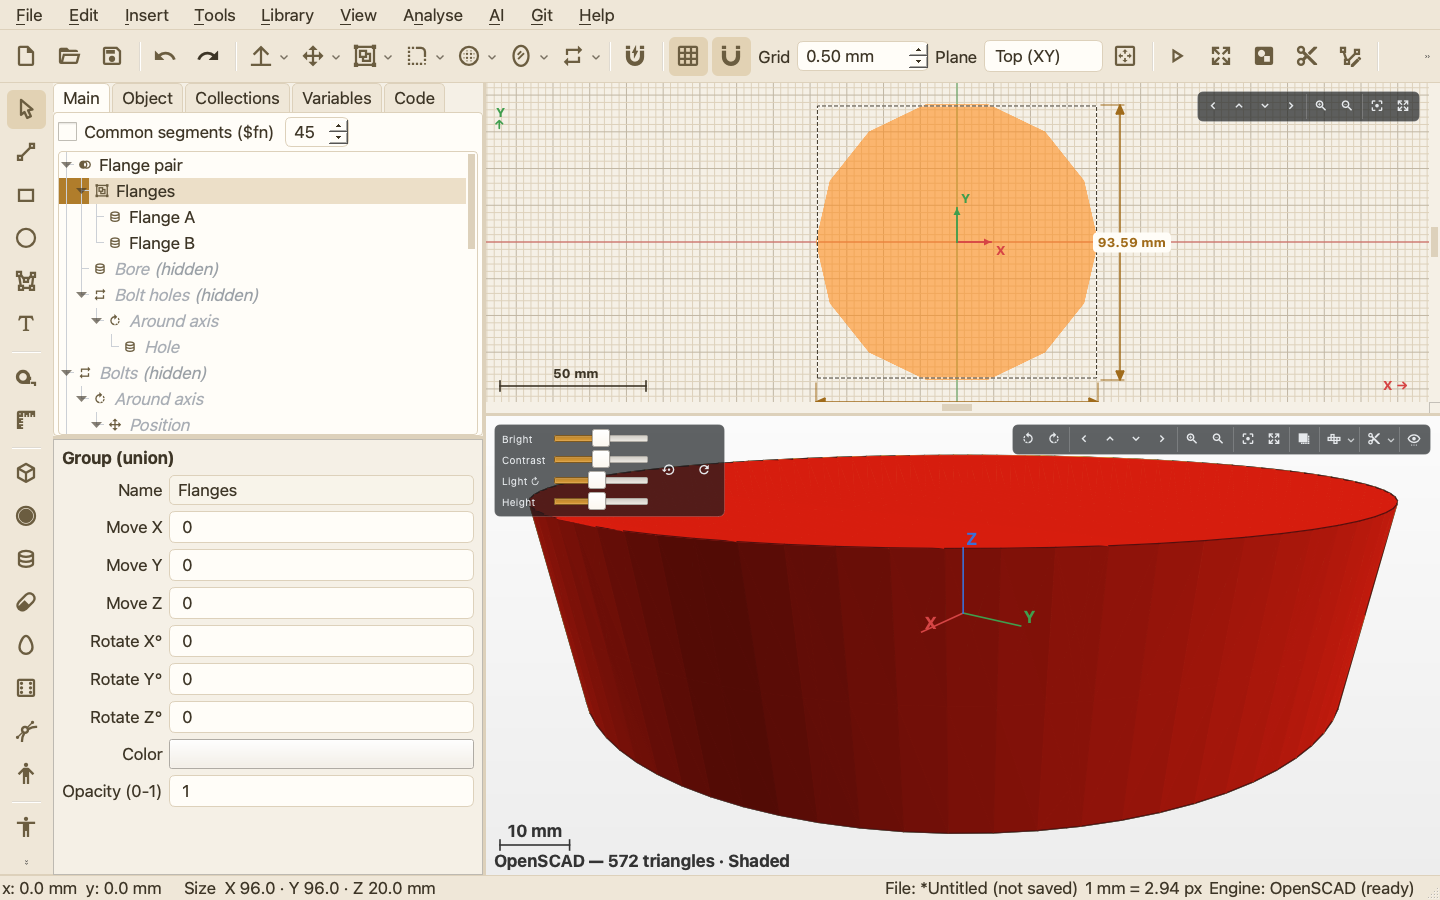
\includegraphics[width=\linewidth]{flange_1_discs.png}\caption{}\end{subfigure}\hfill
\begin{subfigure}{0.49\linewidth}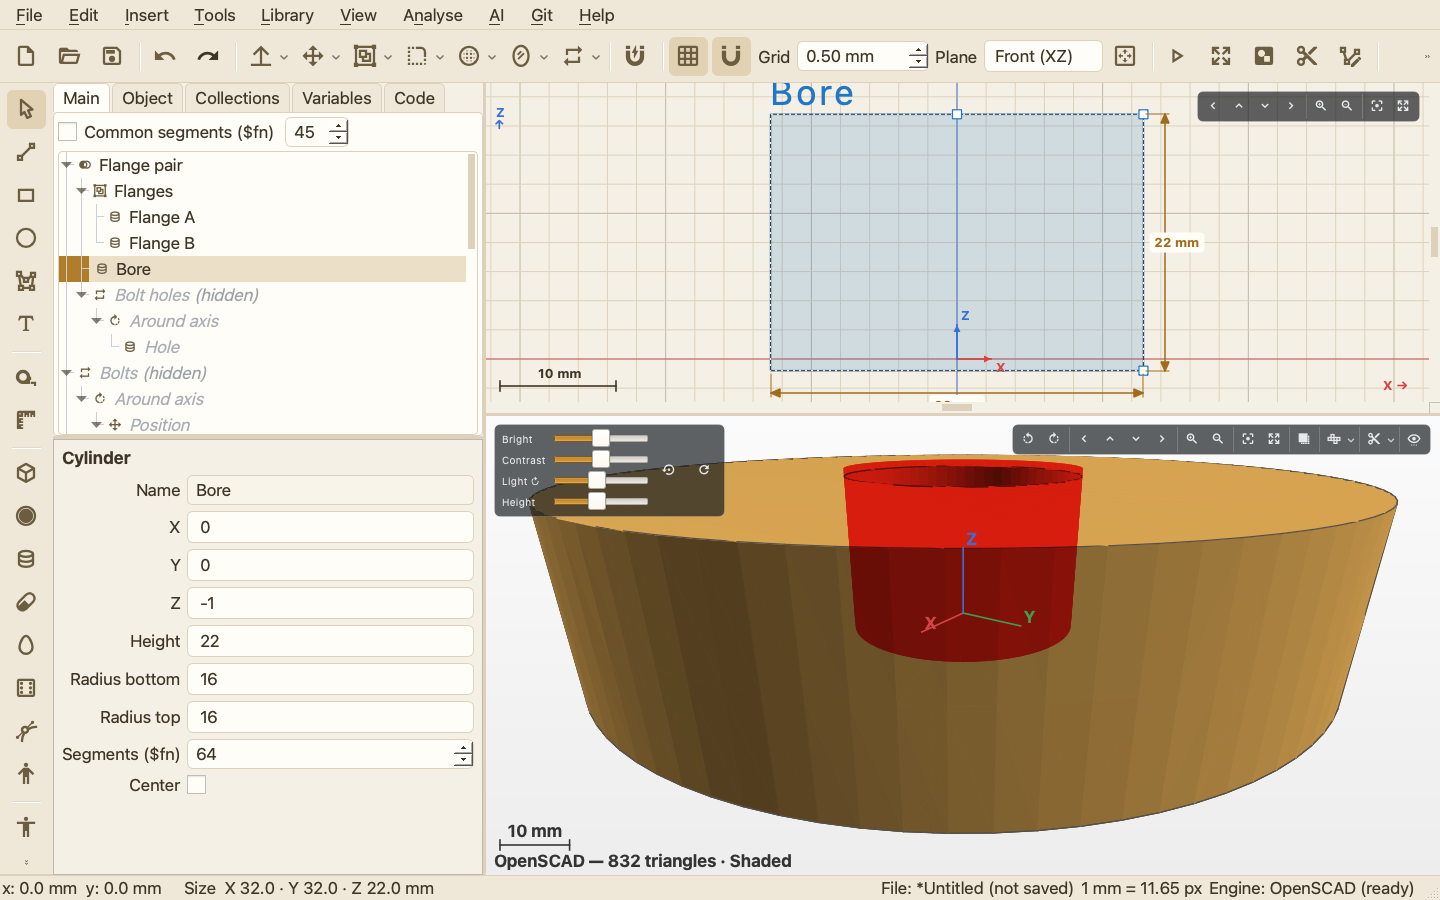
\includegraphics[width=\linewidth]{flange_2_bore.png}\caption{}\end{subfigure}\\[3pt]
\begin{subfigure}{0.49\linewidth}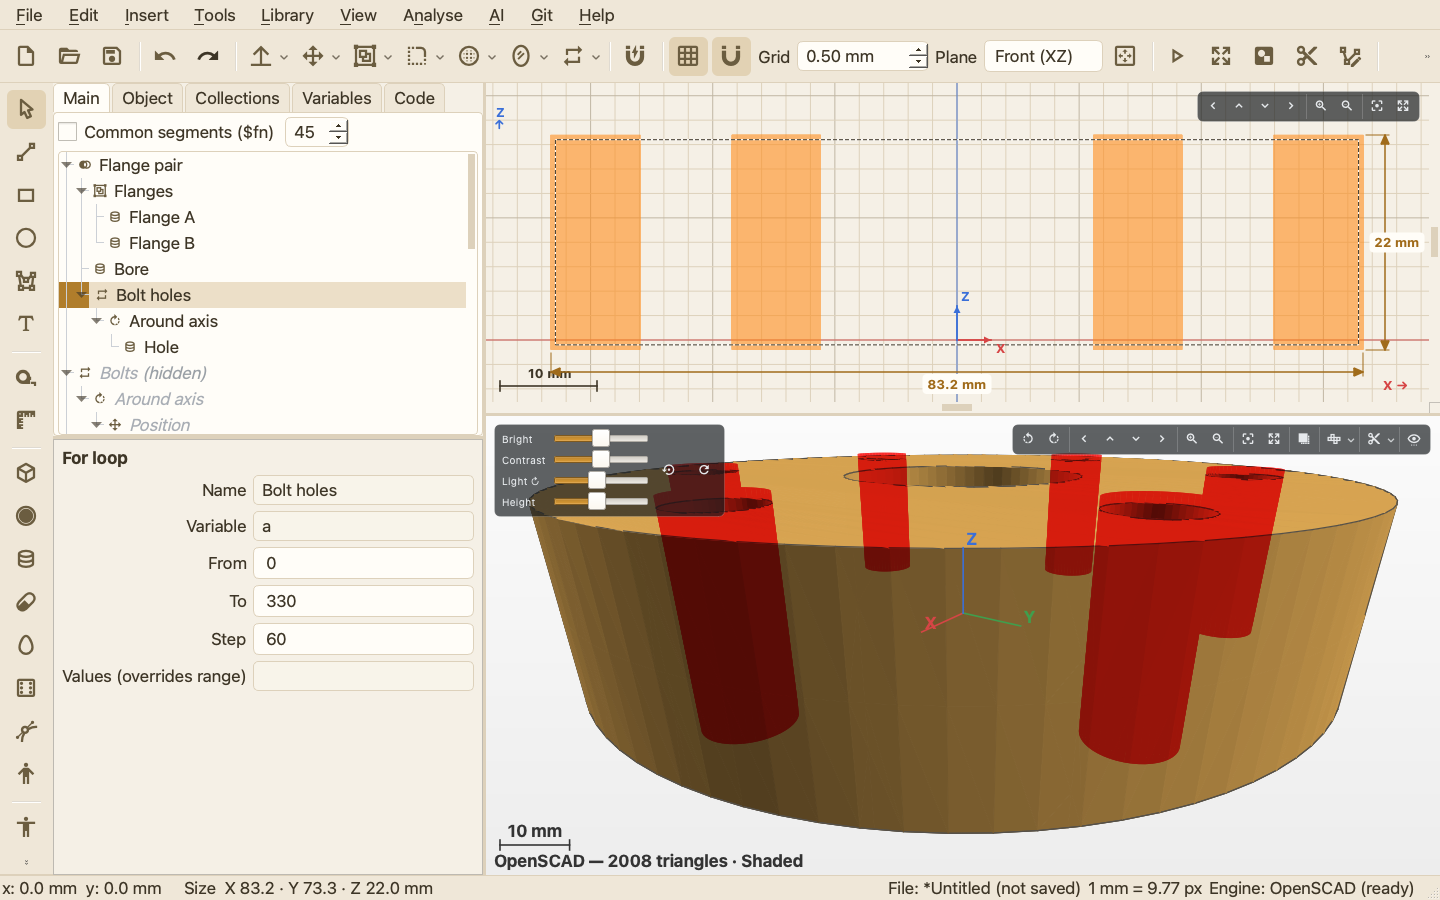
\includegraphics[width=\linewidth]{flange_3_holes.png}\caption{}\end{subfigure}\hfill
\begin{subfigure}{0.49\linewidth}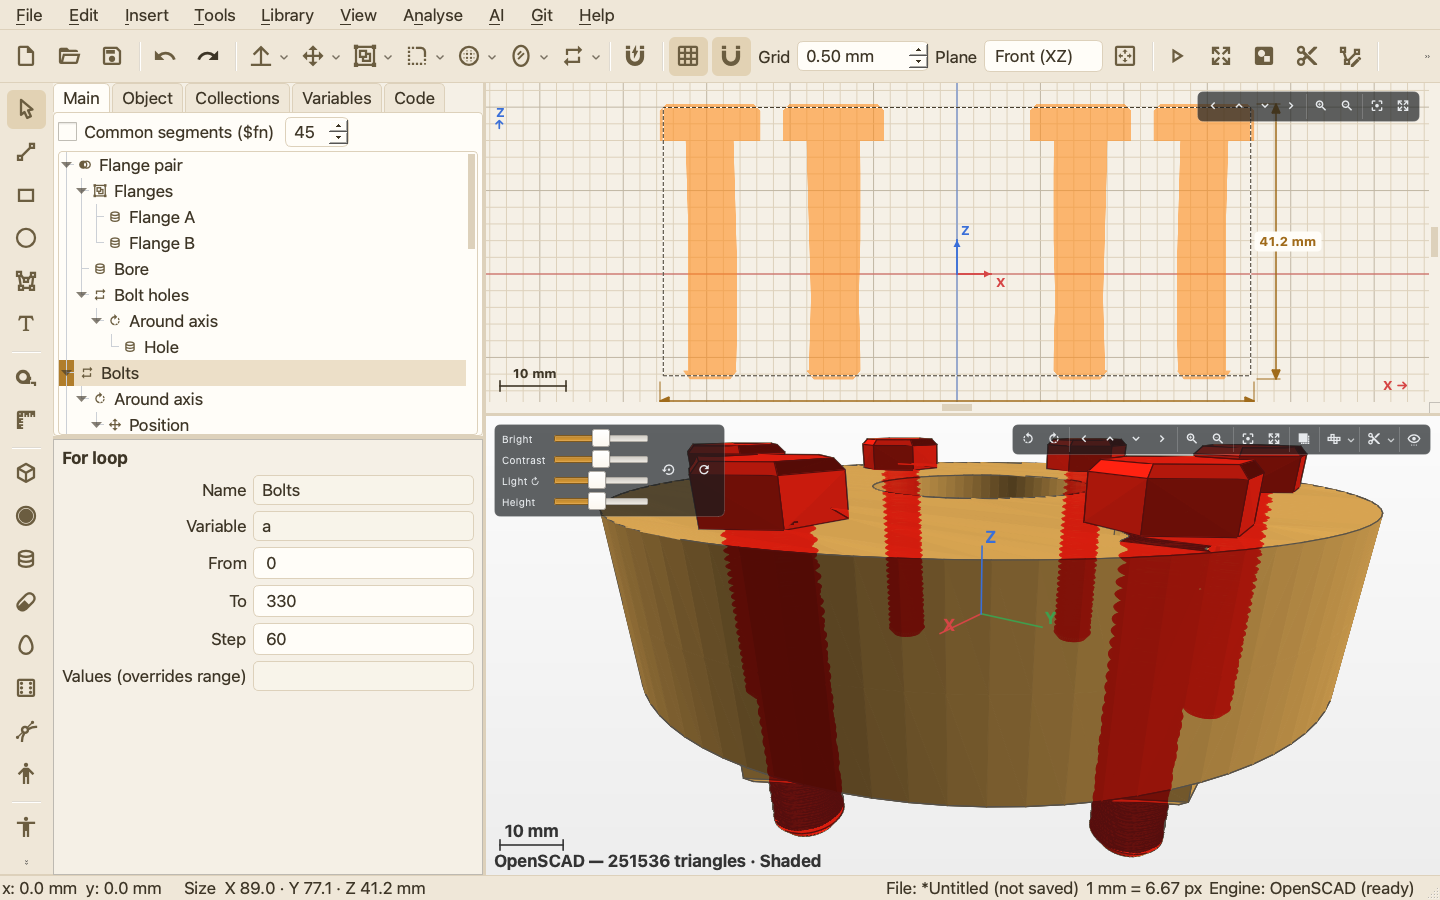
\includegraphics[width=\linewidth]{flange_4_bolts.png}\caption{}\end{subfigure}\\[3pt]
\begin{subfigure}{0.55\linewidth}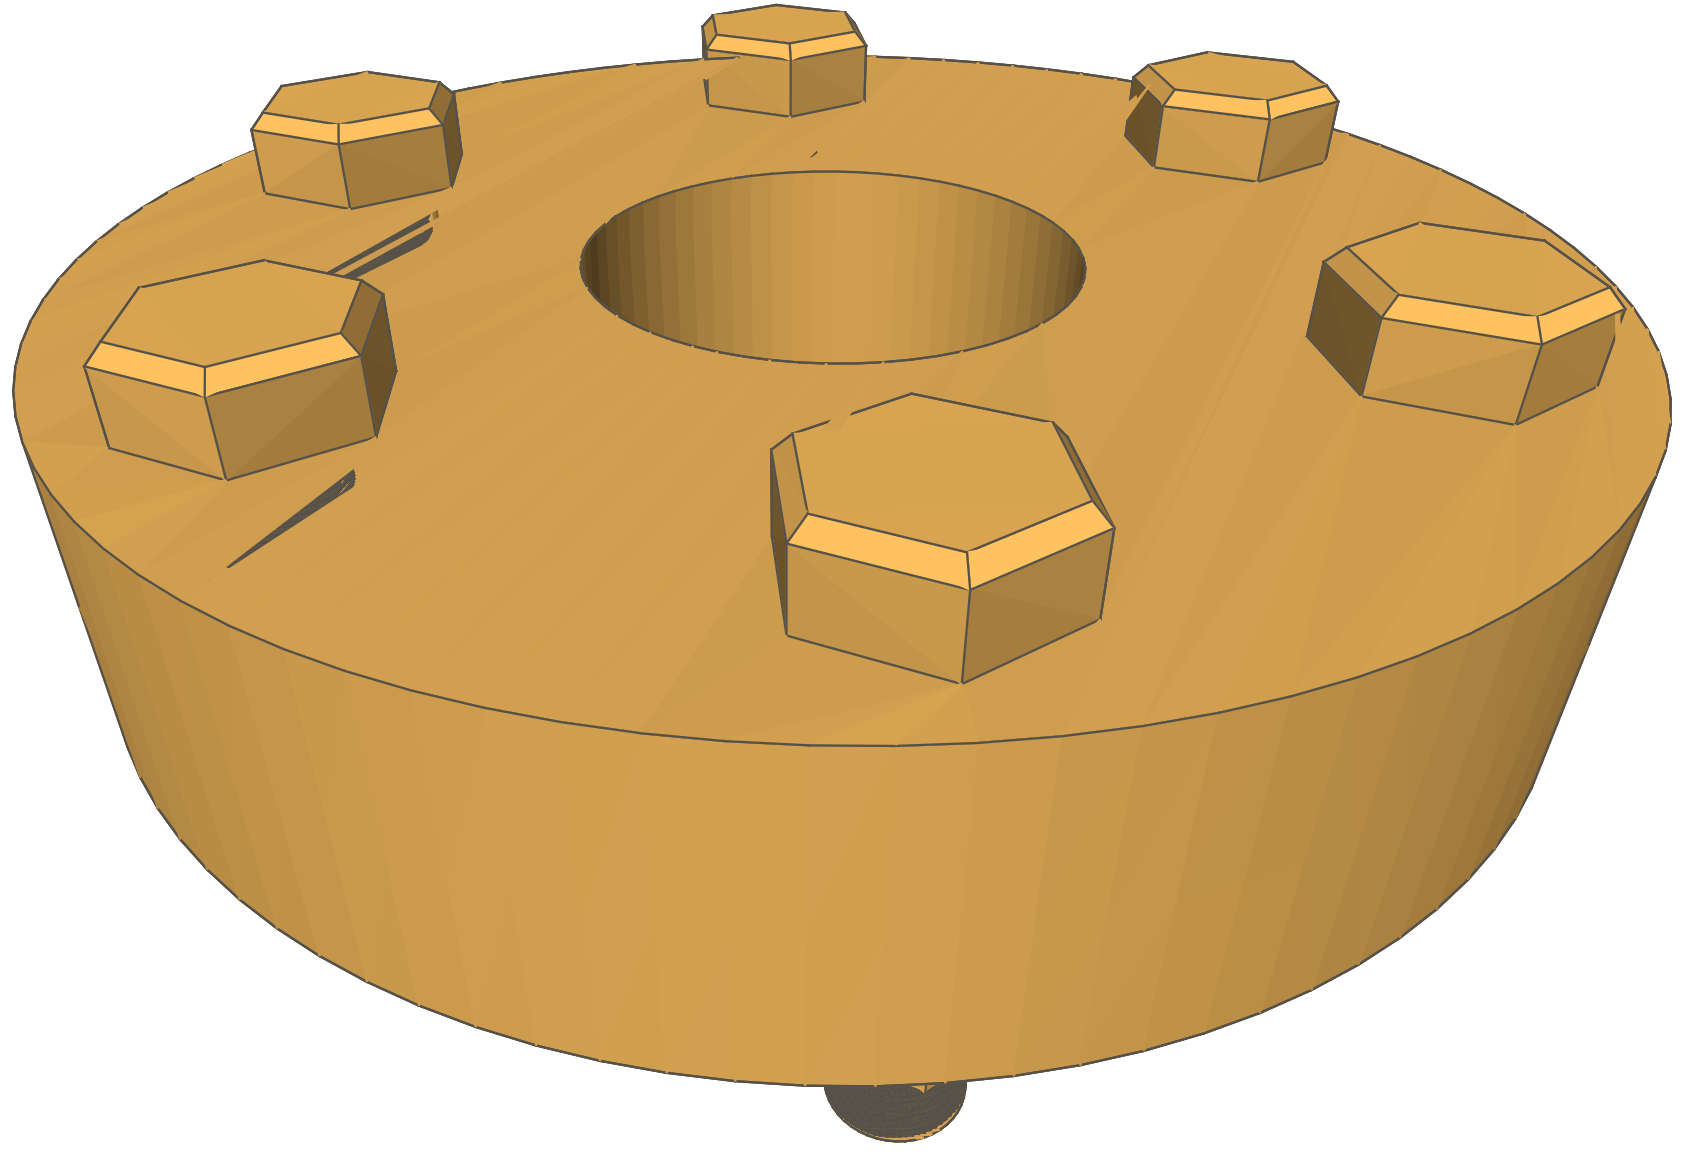
\includegraphics[width=\linewidth]{flange_final.png}\caption{}\end{subfigure}
\caption{A bolted flange joint built node by node: (a) two discs, (b) the bore added to a difference, (c) six bolt holes from one loop, (d) bolts and nuts, (e) the exact OpenSCAD render. The selected node is tinted red.}
\label{fig:flange}
\end{figure}

\subsection{Parts and Assemblies}
An \emph{Object} is a part definition that compiles to an OpenSCAD \texttt{module}; the main tab holds placed instances of Objects. Instances can be mated face to face, concentrically, as a hinge or through a gear ratio, and the mates are solved into ordinary placement parameters, so the program stays plain OpenSCAD. Figure~\ref{fig:hinge} shows a printable butt hinge as three Objects, and Listing~\ref{lst:hinge} the program they produce.

\begin{figure}[t]
\centering
\begin{subfigure}{\linewidth}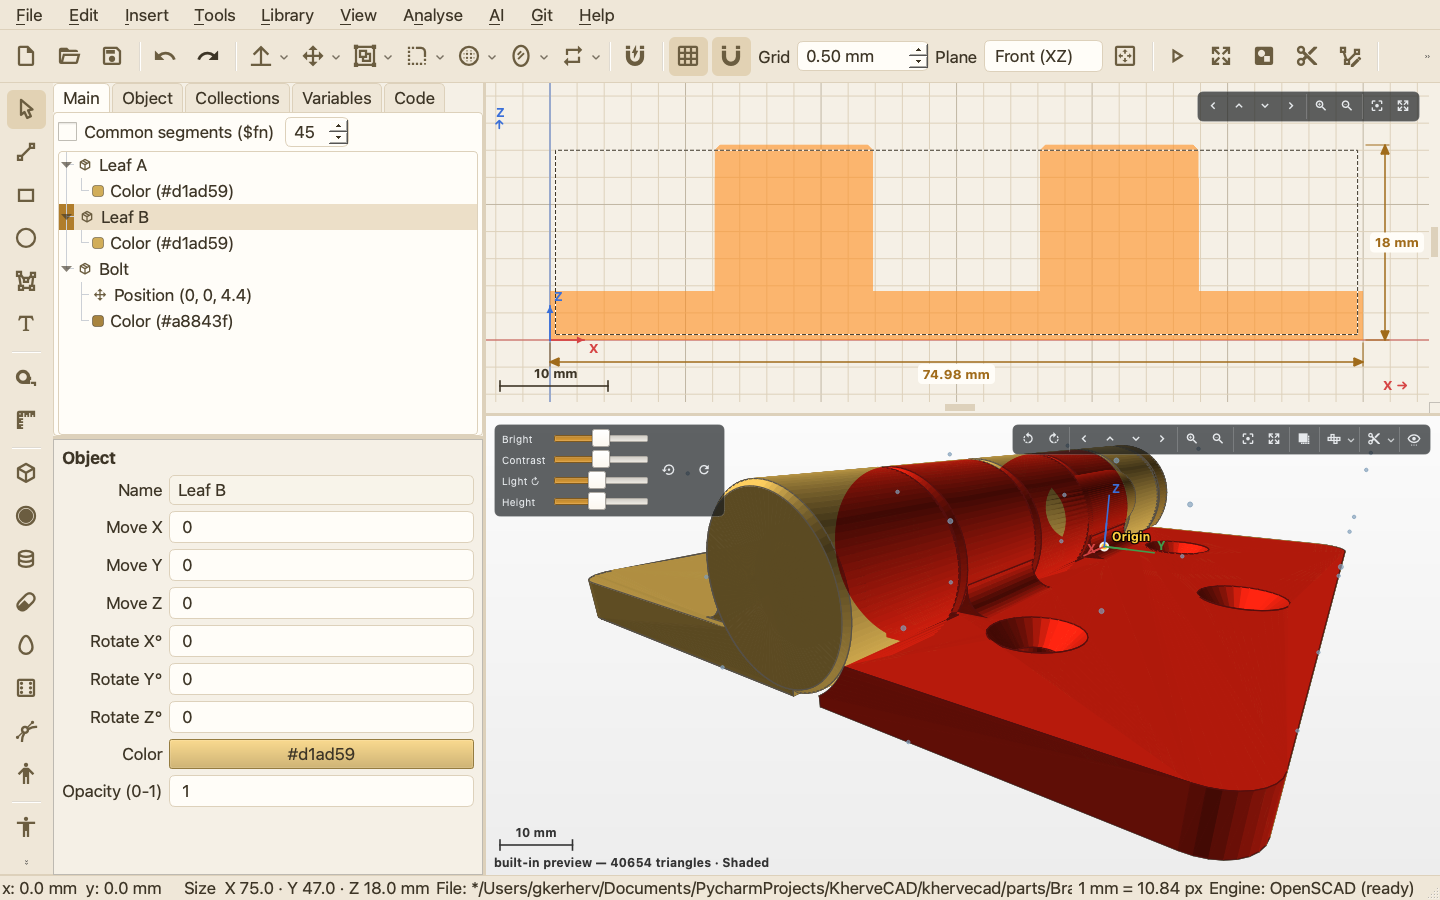
\includegraphics[width=\linewidth]{hinge_tree.png}\caption{}\end{subfigure}\\[3pt]
\begin{subfigure}{0.32\linewidth}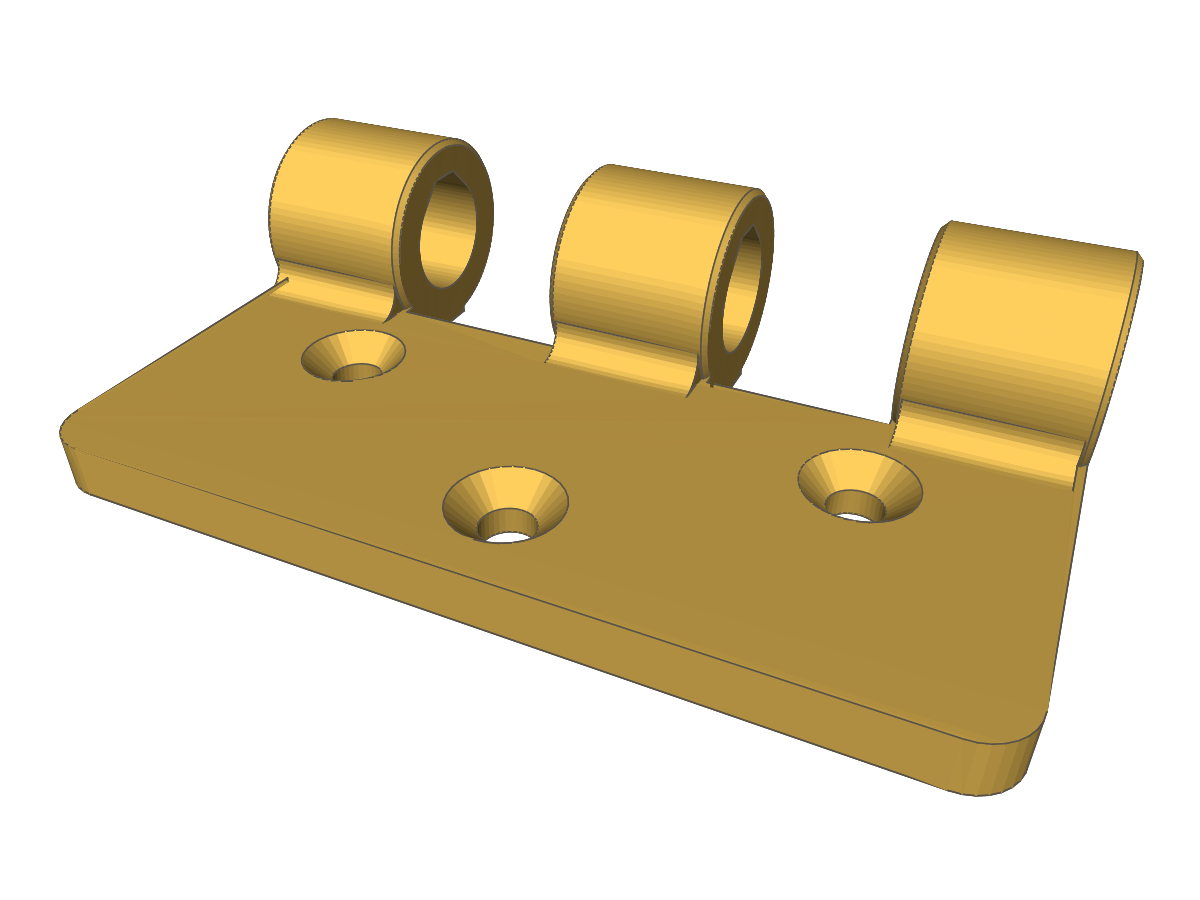
\includegraphics[width=\linewidth]{hinge_Leaf_A.png}\caption{}\end{subfigure}\hfill
\begin{subfigure}{0.32\linewidth}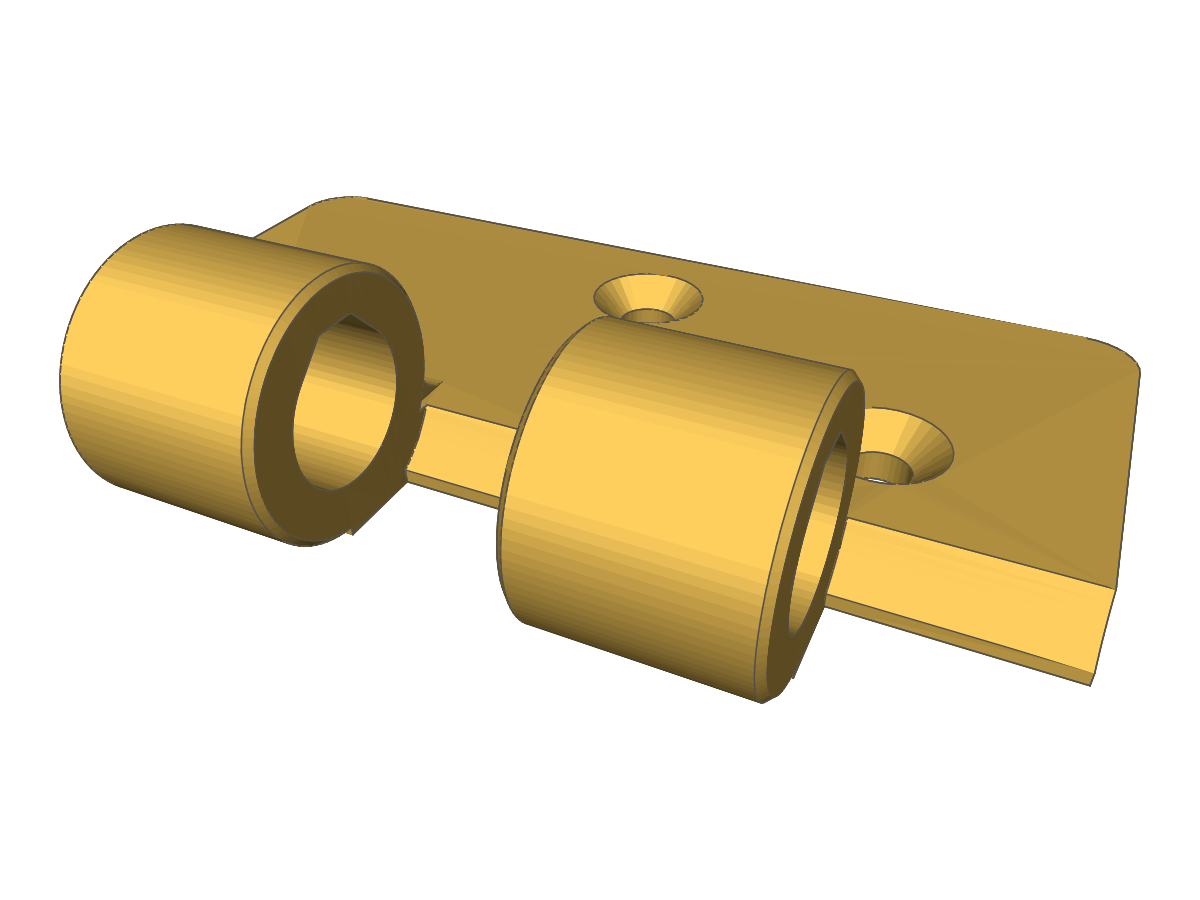
\includegraphics[width=\linewidth]{hinge_Leaf_B.png}\caption{}\end{subfigure}\hfill
\begin{subfigure}{0.32\linewidth}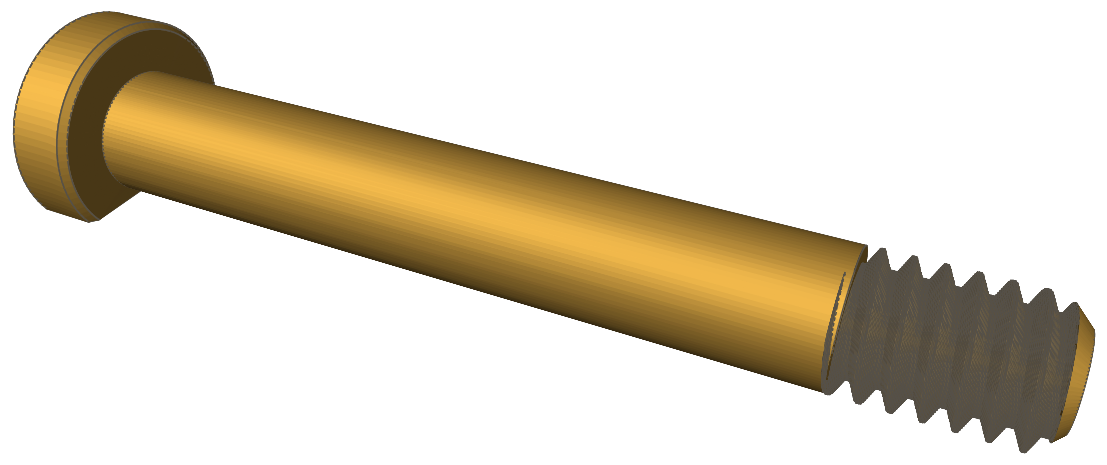
\includegraphics[width=\linewidth]{hinge_Bolt.png}\caption{}\end{subfigure}
\caption{Butt hinge in three printable Objects: (a) the tree, (b) Leaf A, (c) Leaf B, (d) the removable threaded pin.}
\label{fig:hinge}
\end{figure}

\begin{lstlisting}[float=t,caption={Outline of the program generated for the hinge. Each Object is a module and one placed call.},label=lst:hinge]
module Leaf_A() { ... }                                // 97 lines
color("#d1ad59") Leaf_A();  // Leaf A
module Leaf_B() { ... }                                // 74 lines
color("#d1ad59") Leaf_B();  // Leaf B
module Bolt() {
    difference() {
        union() {
            translate([0, 0, 4.6]) rotate([0, 90, 0])        // head
                rotate_extrude($fn=96) polygon(points=[...]);
            translate([-0.5, 0, 4.6]) rotate([0, 90, 0])     // shank
                cylinder(h=59, r1=4.95, r2=4.95, $fn=96);
            translate([58, 0, 4.6]) rotate([0, 90, 0])       // thread
                linear_extrude(height=14.5, twist=-2610, slices=174)
                    polygon(points=[...]);
        }
        translate([-7, -10, -10]) cube([80.5, 20, 10]);      // flat to print on
        translate([-6.01, 0, 4.6]) rotate([0, 90, 0])        // hex socket
            cylinder(h=5.01, r1=3.4641, r2=3.4641, $fn=6);
    }
}
color("#a8843f") translate([0, 0, 4.4]) Bolt();
\end{lstlisting}

\subsection{Geometry}
A Python tessellator draws an immediate preview, with Boolean operations cut by Manifold~\cite{manifold} when it is installed. OpenSCAD then renders each Object separately in the background; the exact mesh replaces the preview as it arrives and is cached by the Object's content. Rendering per part keeps each part's colour and means that moving a part re-renders nothing. Exchange with other CAD systems goes through Open CASCADE~\cite{occt}, which writes exact STEP surfaces for primitives, extrusions, revolutions and Booleans.

\section{The Agent Interface}

\begin{figure}[t]
\centering
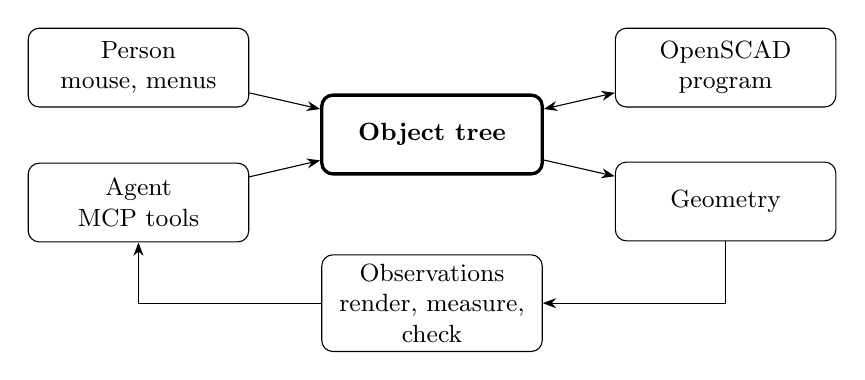
\begin{tikzpicture}[font=\small, box/.style={draw, rounded corners, align=center, minimum width=2.8cm, minimum height=1.0cm}, >=Stealth]
\node[box] (user) {Person\\mouse, menus};
\node[box, below=0.7cm of user] (ai) {Agent\\MCP tools};
\node[box, very thick, right=0.9cm of user, yshift=-0.85cm] (tree) {\textbf{Object tree}};
\node[box, right=0.9cm of tree, yshift=0.85cm] (code) {OpenSCAD\\program};
\node[box, right=0.9cm of tree, yshift=-0.85cm] (geo) {Geometry};
\node[box, below=1.0cm of tree] (chk) {Observations\\render, measure,\\check};
\draw[->] (user) -- (tree);
\draw[->] (ai) -- (tree);
\draw[<->] (tree) -- (code);
\draw[->] (tree) -- (geo);
\draw[->] (geo) |- (chk);
\draw[->] (chk) -| (ai);
\end{tikzpicture}
\caption{The person and the agent edit the same tree; the agent also receives observations of the geometry.}
\label{fig:arch}
\end{figure}

KherveCAD exposes 88 tools through MCP (Fig.~\ref{fig:arch}). Table~\ref{tab:tools} groups them by what they give the agent.

\begin{table}[t]
\caption{Tool groups offered to the agent (selection).}
\label{tab:tools}
\centering\small
\begin{tabular}{p{0.24\linewidth}p{0.68\linewidth}}
\toprule
Group & Examples \\
\midrule
Program & \texttt{apply\_code} (OpenSCAD parsed into nodes; refused if nothing parses), \texttt{get\_code}, \texttt{check\_code} \\
Tree edits & \texttt{add\_node}, \texttt{set\_params}, \texttt{wrap\_nodes}, \texttt{make\_object}, \texttt{attach\_parts} \\
Design-intent actions & \texttt{insert\_part} (library), \texttt{fillet\_edges}, \texttt{push\_pull\_face}, \texttt{split\_part}, \texttt{build\_surface} \\
Seeing & \texttt{render\_view} (image from any camera, after the exact render) \\
Measuring & \texttt{mass\_properties}, \texttt{check\_printability}, \texttt{check\_interference}, \texttt{probe\_surface}, \texttt{measure}, \texttt{section} \\
Documents & \texttt{save\_document}, \texttt{export\_document}, \texttt{export\_drawing} \\
\bottomrule
\end{tabular}
\end{table}

Three design rules shaped the interface. First, every action is an action a person could take, through the same code path; the agent never edits a private copy. Second, each tool call is one undo step, so a person can step back through an agent's work with Ctrl+Z. Third, the agent is told why something failed: parameter names are checked against the node schema, a program that yields no objects is refused rather than silently emptied, and an export that could only be approximated says so. The server listens only on the local machine with a per-session token, and the user chooses whether the agent may read, edit the open document, or also touch files.

\section{Evaluation}

\subsection{Research Questions}
\begin{itemize}
\item[RQ1] Does an agent that can inspect renders produce correct parts more often than one that writes code once?
\item[RQ2] Do numerical observations (mass properties, printability, interference) add to what renders alone provide?
\item[RQ3] Does building into an editable tree, rather than writing a script, change how often the result can be modified afterwards without starting again?
\end{itemize}

\subsection{Tasks}
The benchmark holds [N] tasks in three tiers: single parts with stated dimensions (e.g.\ an L-bracket with two counterbored M5 holes), printable parts with constraints (a hinge with 0.3\,mm clearance and no overhang above 45\textdegree), and assemblies (a flange pair bolted on a pitch circle with no interference). Each task has a written brief, a reference model and an automatic checker.

\subsection{Conditions}
The same model is run in three conditions: \textbf{C0}, code written once and submitted; \textbf{C1}, the agent may call \texttt{render\_view} and revise; \textbf{C2}, the agent may also call the measuring tools. Each task is repeated [k] times per condition, with a budget of [B] tool calls.

\subsection{Metrics}
Success means the result passes every check in the brief. We also report the volume intersection-over-union with the reference, the largest dimensional error, the number of tool calls, wall-clock time, and, for RQ3, whether a follow-up change (``make the plate 5\,mm thicker'') succeeds in one call.

\subsection{Results}
\begin{table}[t]
\caption{Results by condition. [To be filled from the benchmark runs.]}
\label{tab:results}
\centering\small
\begin{tabular}{lcccc}
\toprule
Condition & Success (\%) & IoU & Max error (mm) & Calls \\
\midrule
C0 code once & -- & -- & -- & 1 \\
C1 + renders & -- & -- & -- & -- \\
C2 + measurements & -- & -- & -- & -- \\
\bottomrule
\end{tabular}
\end{table}

[Report Table~\ref{tab:results} and the failure analysis here.]

\section{Applications}

KherveCAD is used to teach CAD modelling: 21 graded tutorials take a student from a single cube to loops and modules, and the code tab shows the program growing with each click. PhD students use its crystal and surface builders to prepare unit cells and slabs; a bulk-terminated surface along any $(hkl)$ is one call and stays an editable program (Fig.~\ref{fig:range}a). The same representation holds a full-size ultra-high-vacuum chamber, which we used to check how a new system would fit in our laboratory, and architectural models such as a Regency town house built with the House Builder (Fig.~\ref{fig:range}).

\begin{figure}[t]
\centering
\begin{subfigure}{0.3\linewidth}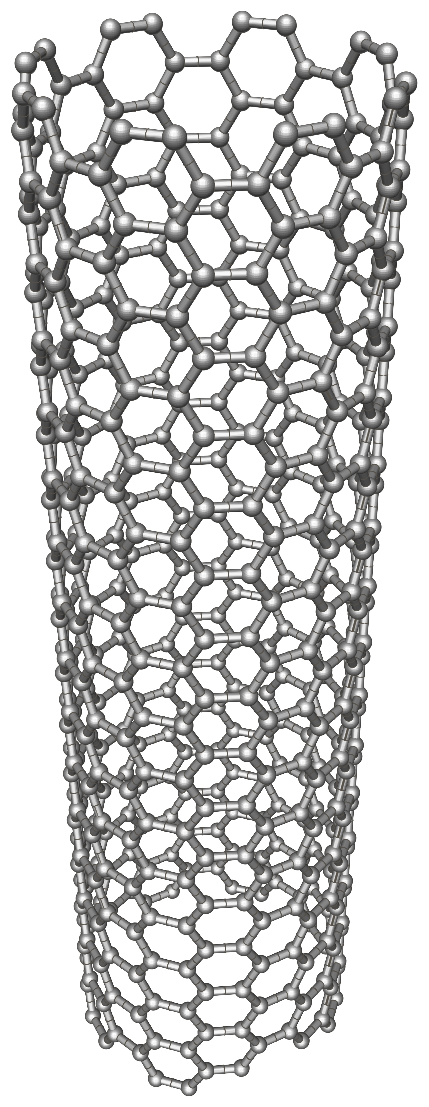
\includegraphics[width=\linewidth]{fig4_nanotube.png}\caption{}\end{subfigure}\hfill
\begin{subfigure}{0.3\linewidth}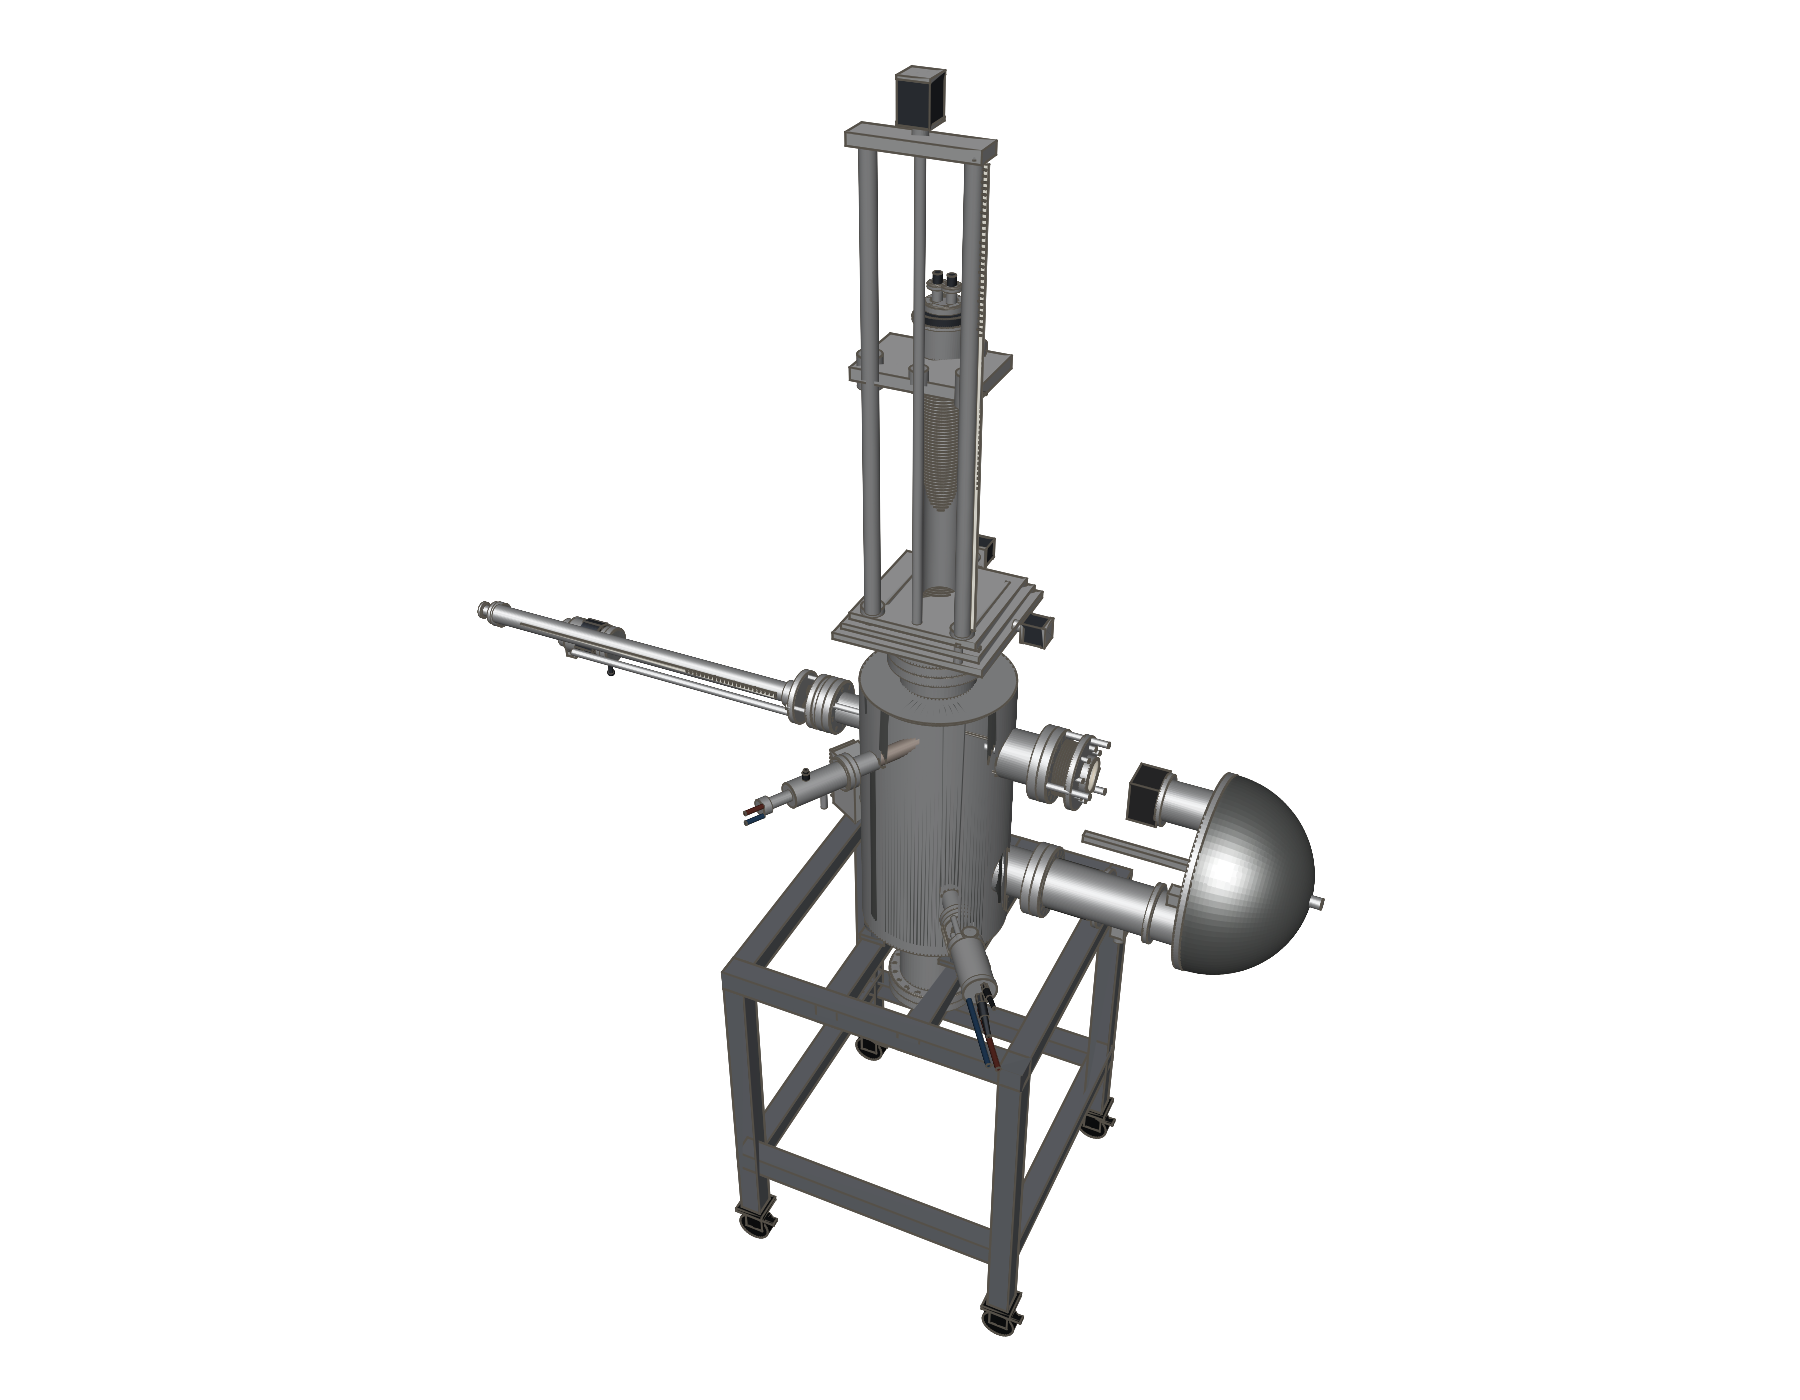
\includegraphics[width=\linewidth]{fig3_chamber.png}\caption{}\end{subfigure}\hfill
\begin{subfigure}{0.36\linewidth}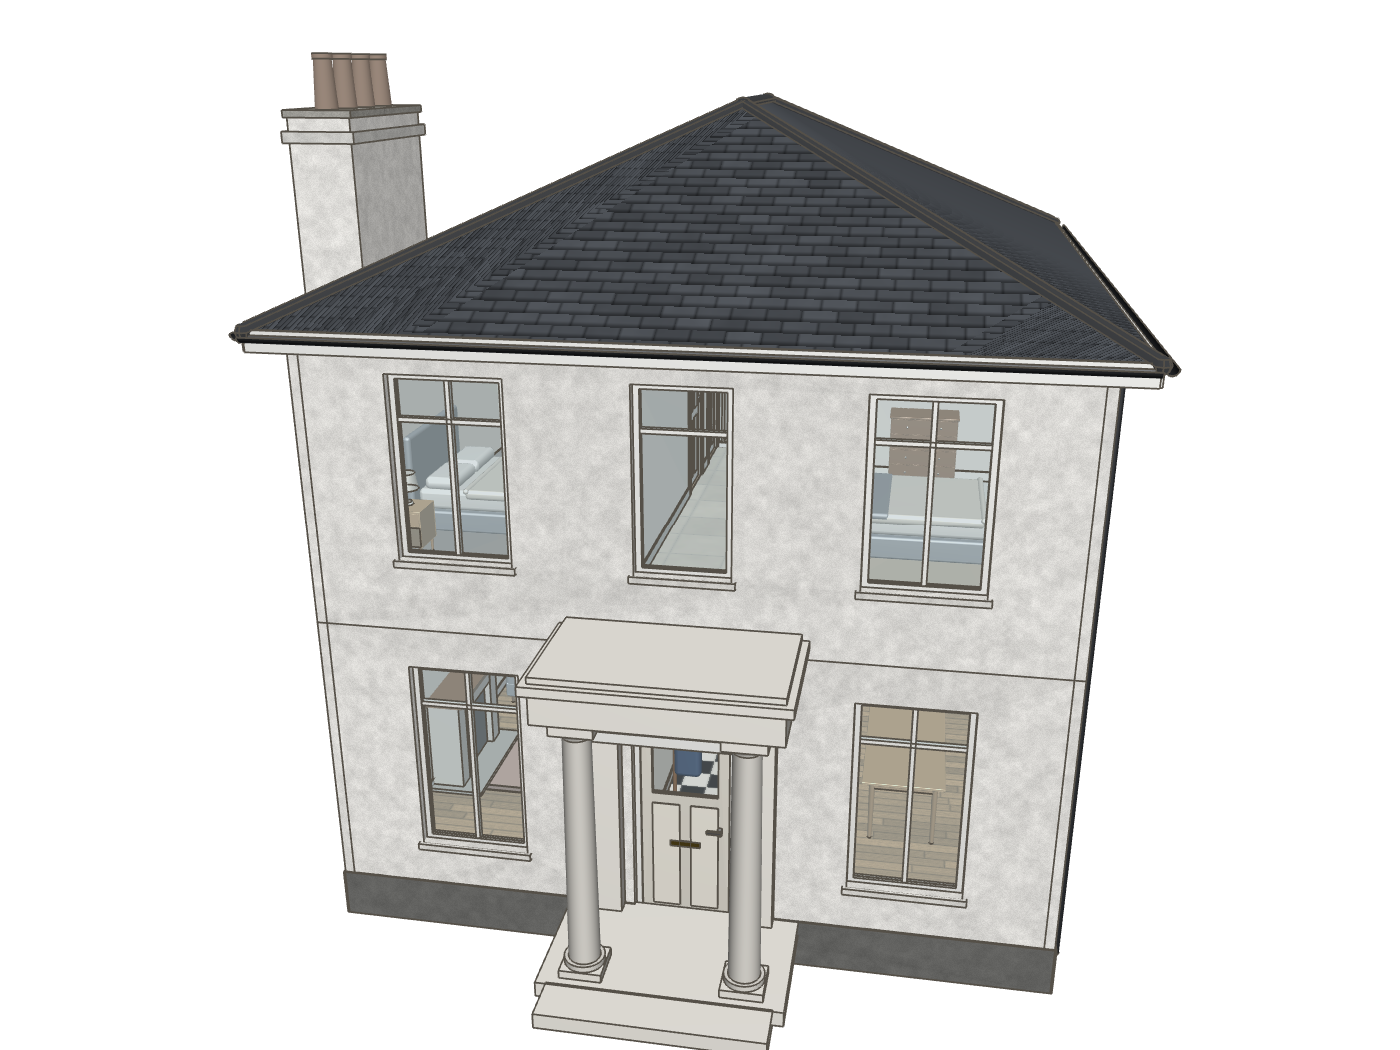
\includegraphics[width=\linewidth]{showcase_regency.png}\caption{}\end{subfigure}
\caption{One representation across scales: (a) a carbon nanotube, (b) a UHV chamber mock-up, (c) a Regency house.}
\label{fig:range}
\end{figure}

KherveCAD is part of KherveTools~\cite{khervetools}, a family of free, open-source applications for scientists that includes KherveFitting~\cite{kerherve2026khervefitting}.

\section{Discussion and Limitations}

The interface makes errors visible; it does not prevent them, and results depend on the model behind the agent. The built-in preview approximates some operations until OpenSCAD has rendered them, so an agent checking too early may measure an approximation; \texttt{render\_view} waits for the exact render by default for this reason. Sketches have no geometric constraint solver yet, so design intent such as ``tangent'' or ``equal'' has to be written as expressions. The benchmark covers mechanical parts and does not test freeform surfaces.

\section{Conclusions}

Giving an agent a CAD system rather than a code box means giving it the same actions a person has, on the same document, together with the observations a person would use to check a part. KherveCAD implements this through a tree that maps one-to-one onto OpenSCAD and an MCP interface of 88 tools. [Restate the measured gain from C0 to C2.] The software and the benchmark are open source.

\section*{Software Availability}
KherveCAD is released under GPL-3.0 at \url{https://github.com/gkerherve/KherveCAD} and archived on Zenodo~\cite{kherveCADzenodo}.

\begin{acknowledgment}
[To fill in.]
\end{acknowledgment}

\section*{Declaration of Generative AI Use}
The author used Claude (Anthropic) to help write code and draft text, and reviewed and edited all content.

\bibliographystyle{asmejour}
\bibliography{references}

\end{document}
